%Copyright 2014 Jean-Philippe Eisenbarth
%This program is free software: you can 
%redistribute it and/or modify it under the terms of the GNU General Public 
%License as published by the Free Software Foundation, either version 3 of the 
%License, or (at your option) any later version.
%This program is distributed in the hope that it will be useful,but WITHOUT ANY 
%WARRANTY; without even the implied warranty of MERCHANTABILITY or FITNESS FOR A 
%PARTICULAR PURPOSE. See the GNU General Public License for more details.
%You should have received a copy of the GNU General Public License along with 
%this program.  If not, see <http://www.gnu.org/licenses/>.

%Based on the code of Yiannis Lazarides
%http://tex.stackexchange.com/questions/42602/software-requirements-specification-with-latex
%http://tex.stackexchange.com/users/963/yiannis-lazarides
%Also based on the template of Karl E. Wiegers
%http://www.se.rit.edu/~emad/teaching/slides/srs_template_sep14.pdf
%http://karlwiegers.com

%Modified for EECS 393 project in Spring 2017
%Dina Benayad-Cherif, Jason Dong, Mark Lalor, Yousef Mahmoud, Vimig Socrates
\documentclass[16pt]{scrreprt}
\usepackage{longtable}
\usepackage[T1]{fontenc}
\usepackage[utf8]{inputenc}
\usepackage{float}
\usepackage{graphicx}
\usepackage{makecell}
\usepackage{listings}
\usepackage{xcolor}
\usepackage[bookmarks=true]{hyperref}
\usepackage[english]{babel}
\usepackage[utf8]{inputenc}
\usepackage[english]{babel}

\hypersetup{
    bookmarks=false,
    pdftitle={Software Design Document},
    pdfauthor={Dina Benayad-Cherif, Jason Dong, Mark Lalor, Yousef Mahmoud, Vimig Socrates},
    pdfsubject={EECS 393 Software Design Document},
    pdfkeywords={SRS, Software, Design},
    colorlinks=true,        % false: boxed links; true: colored links
    linkcolor=blue,         % color of internal links
    citecolor=black,        % color of links to bibliography
    filecolor=black,        % color of file links
    urlcolor=purple,        % color of external links
    linktoc=page            % only page is linked
}

\addto\captionsenglish{\renewcommand{\contentsname}{Table Of Contents}}
\def\myversion{1.0}
\date{}

\begin{document}

% Title Page
\begin{flushright}
	\rule{16cm}{5pt}\vskip1cm
	\Huge{SOFTWARE DESIGN\\ DOCUMENT}\\
	\vspace{0.3cm}
	for\\
	\vspace{0.4cm}
	iSport\\
	\begin{figure}[H]
		\flushright
  		
\includegraphics[width=.2\textwidth]{diagrams/logo.png}
		\end{figure}
	\normalsize{Release \myversion \\}
	\vspace{1cm}
	Prepared by\vspace{0.5cm} \\ 
        \normalsize{1650940 Jiang Xiaohu\\1650932 Xu Jingnan\\1651058 Wang Yicheng}
        \\
        \vspace{1.1cm}
        \normalsize{School of Software Engineering\\ Tongji University}\\
        \vspace{1.0cm}
        \today
	\vfill
	\rule{16cm}{5pt}
\end{flushright}

\tableofcontents

\chapter*{Revision History}

\begin{center}
    \begin{tabular}{|p{5cm}|p{3cm}|p{7cm}|p{2cm}|}
        \hline
	    Name & Date & Reason For Changes & Version\\
        \hline
	    Jiang Xiaohu & 2019.11.12 & Finish Introduction Part  & v1.0\\
        \hline
	    Wang Yicheng & 2019.11.14 & Finish Overview Part & v1.1\\
        \hline
        Xu Jingnan & 2019.11.16 & Finish External Requirements Part & v1.2\\
        \hline
        Xu Jingnan, Jiang Xiaohu, Wang Yicheng & 2019.11.18 & Finish Sequence Diagrams for Function Modeling Part& v1.3\\
        \hline
        Xu Jingnan & 2019.11.20 & Finish Function Modeling Part & v1.4\\
        \hline
        Jiang Xiaohu & 2019.11.21 & Finish Data Modeling Part  & v1.5\\
        \hline
        Wang Yicheng & 2019.11.22 & Finish Behavior Requirements Part & v1.6\\
        \hline
        Xu Jingnan & 2019.11.23 & Finish Nonfunctional Requirements Part & v1.7\\
        \hline
        Jiang Xiaohu & 2019.11.25 & Finish Data Dictionary Requirements Part & v1.8\\
        \hline
    \end{tabular}
\end{center}
%%%%%%%%%%%%%%%%
% INTRODUCTION %
%%%%%%%%%%%%%%%%

\chapter{Introduction}

\section{Purpose}
This design document describes the overall structure of iSport by outlining significant aspects of the system’s architecture.\\

\noindent  The purpose of this document is to present a detailed description of iSport. It shows how the software system will be structured to satisfy the requirements.


\section{Scope}
This software system will be a web based system for sports fans, professional athletes, and patients who are under recovering training. \\
\\
This system will be designed to maximize the exercising efficiency by providing tools to assist in checking and correcting user's wrong postures and recommending training courses customized for users, which would otherwise have to be expensive, time-consuming and labor intensive. By maximizing the user’s training efficiency and convenience the system will meet the needs of sports fans, athletes and injured patients while remaining easy to understand and use.\\
\\
More specifically, this system is designed to allow a user to imitate the standard exercising postures while observe and correct their mistakes simultaneously with the help of a website. \\
\\
The software will collect some professional courses in the database, including static and dynamic trainings which means doing exercise according to a set of images or a video and iSport will recommend suitable trainings for users on the basis of their training performance. Courses are classified into exercising courses and recovering courses, aiming to help athletes and patients respectively.\\
\\
Both visual and audio notification are used in every course of the system to provide eye-catching, user-friendly and clear instructions; the feedback of one's training is proposed once the training is over and the report can be browsed in the report page.\\
\\
The selection and deletion of one user's favorable course is supported in personal information webpage and one can comment training he/she has taken on comment webpage to provide suggestions to other users.\\
\\
 The personal information registering, changes is allowed via the application options. The system also contains a relational database containing a list of users, training images and videos.

\section{Acronyms, Abbreviations and Definitions}
\begin{longtable}{|p{1.9in}|p{4in}|c|}
xxxxx & xxxxxx  \kill
\caption{Definitions\label{simple}}\\ \hline
\multicolumn{3}{|c|}{\bf Definitions, Acronyms, and Abbreviations}\\ \hline
\endfirsthead
\caption[]{(continued)}\\ \hline
\multicolumn{3}{|c|}{\bf Definitions, Acronyms, and Abbreviations (continued)}\\
\hline
\endhead
\hline
\multicolumn{3}{|c|}{\bf Continued $\ldots$}\\
\hline
\endfoot
\hline
\multicolumn{3}{|c|}{\bf The End}\\
\hline
\endlastfoot
Term & Definitions  \\
\hline
User & Someone who interacts with iSport including sports fans, athletes and  injured patients who need recovery training.\\  \hline  
Sports fans & One of iSport's potential customers who love sports and want to get professional instructions when exercising. Some of them may can't afford the expense of personal coaching or don't have time to go to the gym. \\ \hline
Athletes & One of iSport's potential customers who want to get real-time exercising feedback to improve their performance or who want to get some relaxing training in their spare time to keep a good competitive state.\\  \hline
Injured Patients & One of iSport's potential customers who need recovering training after some treatments, e.g. surgeries. On the one hand, some of them may can't afford the doctor's expensive medical instructions for recovering training. on the other hand, there is no enough doctors or nurses who can instruct and supervise the patients' recovering exercising. But without professional instructions training can be useless or even leads to secondary trauma.\\  \hline
Admin/Administrator & System administrator who is given specific permission for managing and controlling the system, e.g. updating the user's information, uploading new training courses.\\ \hline
User Info & User's basic information including user's avatar, account name, tel-number and email address.\\ \hline
Courses & Training courses including normal exercising training and recovering training.\\ \hline
Exercise Courses & Training courses which serve the sports fans and athletes.\\ \hline
Recover Courses & Training courses which serve the injured patients.\\ \hline
Static Courses & Training courses which instruct the users photo by photo.\\ \hline
Dynamic Courses & Training courses which instruct the users according to a standard video.\\ \hline
Appraisal Subsystem & Remark the user's performance by using a grade from 0 -100\\ \hline
Comment Subsystem & User comment on the training courses they have taken to provide reference for other users.\\ 
\hline 
Recommendation Subsystem & A subsystem which will provide some courses for users according to their recent performance.\\ 
\hline
Exercise Tips & There will be sports tips in the webpage of iSport to prevent users from athletic injuries.\\ 
\hline 
Sport Report & A web page to feedback the user's exercising performance.\\ 
\hline 
Audio Notification & An audio notification will be shown when the user is doing exercise to encourage the user to hold on or notify the user to correct their postures.\\ 
\hline 
Visual Notification & A visual notification will be shown when the user is doing exercise, if the user's posture is standard, then the web-frame will turn green to suggest the user to hold on, otherwise the web-frame will be red.\\ 
\hline 
DataBase & A relational database containing a list of user info, training images and videos.\\ 
\hline 
Detection Subsystem & Subsystem to detect the user's postures and draw the user's skeleton. The main model of detection subsystem is PoseNet.\\ 
\hline 
Comparison Subsystem & Subsystem to compare the postures of the user and that of the standard. The subsystem aims to check if the user pass the posture.\\ 
\hline 
Correction Subsystem & Subsystem to calculate where the postures' wrong part are, e.g. left-arm, right-leg, head.\\ 
\hline 
Clients & Group who delegate the development of iSport to the developers and will take charge of the later management of iSport.\\ \hline
Developers & Develop team including project managers, programmers, testers who are responsible for the development of iSport and its later mainteinance and updating.\\ 
\hline 
\end{longtable}

\section{Overview}
This document is an overview of the software architecture of iSport in high detail. We start by providing all the principal components that the application is built on as well as their responsibilities to the success of the application. Next, we provide diagrams to show the hierarchy of our classes and the architectural design. Finally, we develop a general API of the major class methods used to build the functionality of our application. There are also mockups of our UI design included in our design document. 

\section{Reference Material}
\subsubsection{Standard References}
The standards we have followed are as follows:\\

$[1]$ T. Russell, A. Brizee, E. Angeli, and R. Keck, “Mla formatting and style guide,” The Purdue OWL, 2010.\\

$[2]$ Barnard, H Jack and Metz, Robert F and Price, Arthur L et al., A recommended practice for describing software designs: IEEE standards project 1016, 1986.\\

$[3]$ R. S. Pressman, Software engineering: a practitioner’s approach. Palgrave Macmillan, 2005.\\

\subsubsection{Writing Tools References}
The writing tools we have used are as follows:\\

$[4]$ L. Lamport, LATEX: a document preparation system: user’s guide and reference manual. Addison-wesley, 1994.\\

$[5]$ S. Wong, “Staruml tutorial,” Connexions Web site, Sep, 2007.\\

$[6]$ P. O. Team, “Process on tools,” https://www.processon.com/support.

%%%%%%%%%%%%%%%%%%%
% SYSTEM OVERVIEW %
%%%%%%%%%%%%%%%%%%%

\chapter{System Overview}
\section{Product Perspective}

ISport is a web system developed by isport team, aimming at posture correcting with the assist of camera.\\

The user-case diagram in the folowing figure illustrates the user-case in the system. The system is expected to evolve over at least three releases, ultimately allowing for complete streamlining of the posture correcting process, fitness classes and rehabilitation classes for learning.

\begin{figure}[H]
	\centering
	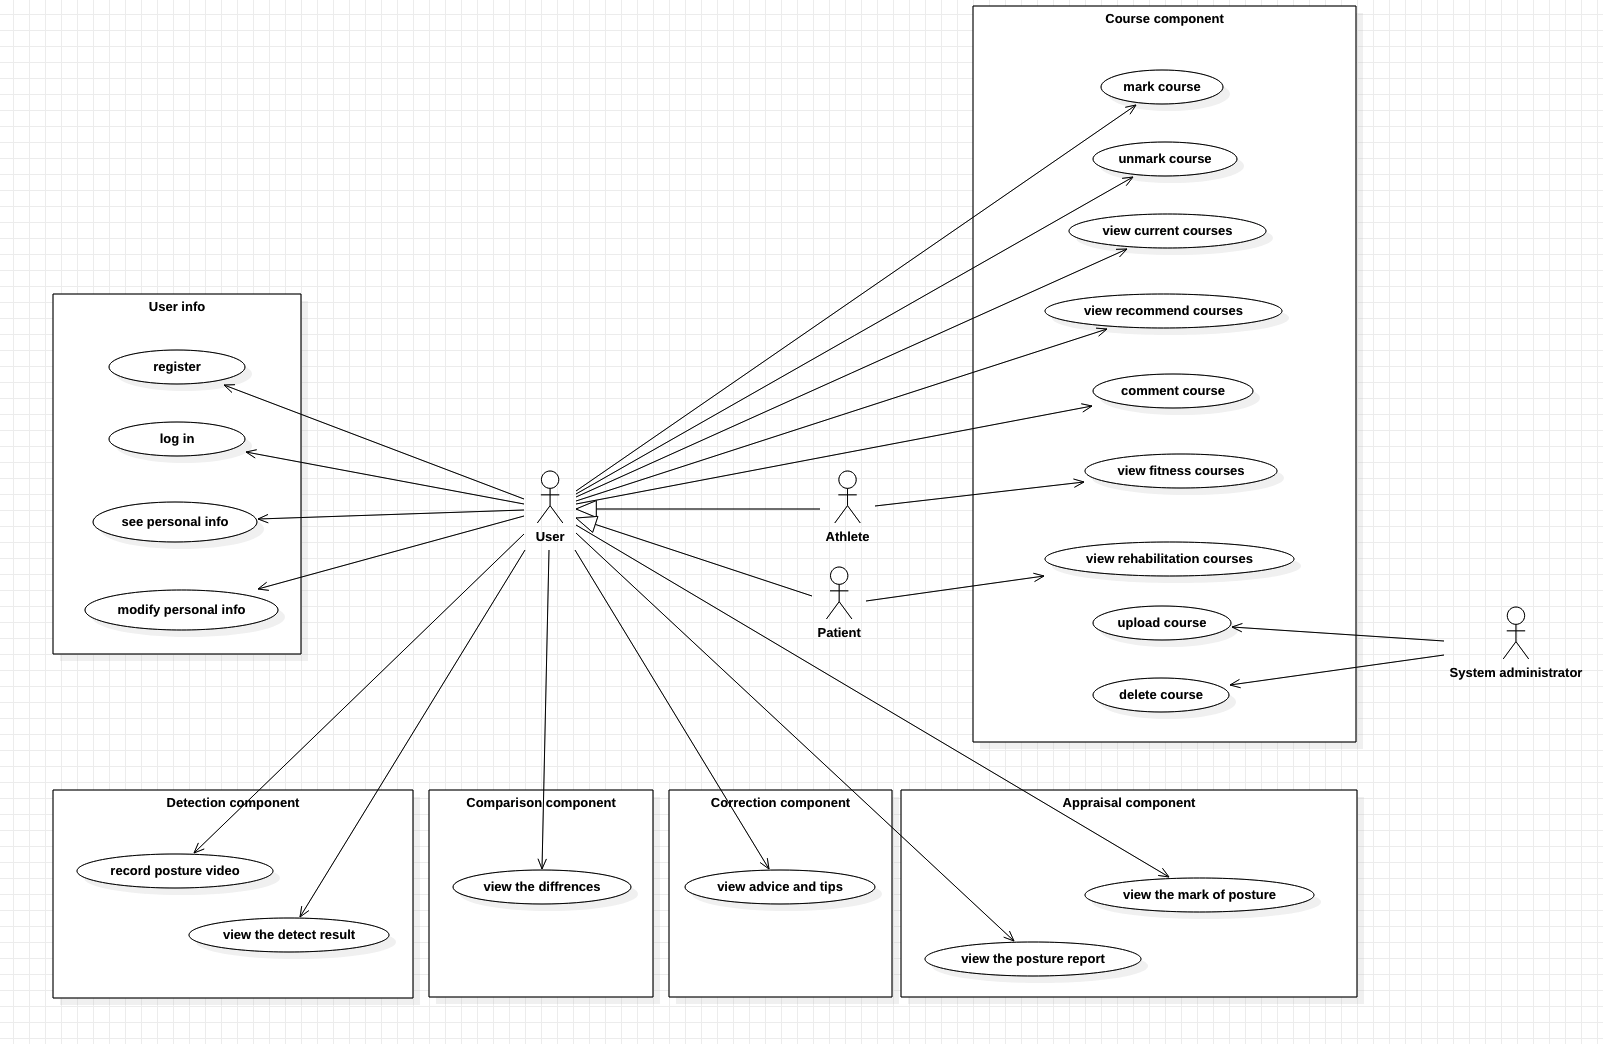
\includegraphics[width=1.0\textwidth]{diagrams/big-user-case.png}
	\caption{overall user-case diagram}
\end{figure}



\section{Product Functionality}

ISport contains these following key features:\\

Let the user register their account of the website through their mobile phone or e-mail.\\

 
Let the user log in to the system by correctly complete the log-in form. If the username is not in the database, the user will be prompted to register his/her account.\\

 
User can modify his/her account information after logging in, including the username, e-mail address, phone number, gender, age and so on.\\

 
Show all the sorted fitness courses in a list for user to choose in the fitness courses view page. \\

 
Show a list of courses that the user has selected to learn before\\

 
Show a list of recommended courses for the user by user's previous behavior \\

 
Show the comment and evaluation of each courses in their detailed page\\

 
Provide the add button for user to add a course he/she want to learn in the future and add the course to his/her courses list.\\

 
Provide the delete button for user to remove a course he/she doesn't want to learn and remove the course from his/her courses list.\\


Generate user's exercise report for watching and analyzing in the report page\\
 
Give the user a space to leave his/her evaluation about the courses learnt before\\

Capture and Collect the posture data of the user in front of the computer and store the data in the server.\\


Compare user's posture with the standard one and calculate the similarity between the postures.\\


Show tips on the user's screen to notice the wrong posture of the user and help to correct them.\\


Rate the user's posture on a scale of zero to ten to let the user know whether his posture is standard or not\\


System administrator can upload new courses to the system for users to choose and learn.\\

\section{Users and Characteristics}

 
\begin{center}
    \begin{tabular}{p{5cm}p{11cm}}
        \hline
	    Users & Desc\\
        \hline
	    People who want to correct their posture &  Normal user is expected to register and log in the system, upload their posture and get the feedback advice from the system\\
        \hline
	    People who want to be fitness & People who want to be fitness is expected to register and log in the system, choose fitness classes for themselves and learn it on the website\\
        \hline
        People who need rehabilitation & People who need rehabilitation is expected to register and log in the system, choose fitness classes for themselves and learn it on the website\\
        \hline
        System Administrator & System Administrator has the privilege to update posture information in the database. The Administrator does not directly interact with the website\\
        \hline
    \end{tabular}
\end{center}

 
\section{Operating Environment}

 
\subsubsection{Hardware}

 
\noindent1. Server\\

 
CPU: Intel Dual-Core 2.4GHz\\

 
Memory: 8GB\\

 
External Storage: 500G SSD\\

 
Quantity: 1\\

 
\noindent 2. Client(Minimum Configuration)\\

 
CPU: Single-Core 1GHz\\

 
Memory: 2G\\

 
External Storage: 20GB HDD\\

 
\subsubsection{Software}

 
\noindent 1. Server\\

 
Operating System: Ubuntu 18.04 LTS\\

 
Database: MySQL\\

 
Software and Library : Python, Spring, TensorFlow, Nginx\\

 
\noindent 2. Client\\

 
Operating System: Windows/macOS/Linux/Android/IOS\\

 
Software: Browser\\

 
\begin{center}
    \begin{tabular}{p{7cm}p{7cm}}
        \hline
	    Recommand Browser & Version\\
        \hline
	    Google Chrome &  44+\\
        \hline
	    Mozilla Firefox & 40+\\
        \hline
        Apple Safari & 7+\\
        \hline
        Microsoft Edge & 12+\\
        \hline
        Microsoft Internet Explorer & 11+\\
        \hline
        Opera Opera & 31+\\
        \hline

 
    \end{tabular}
\end{center}

 
\section{Design and Implementation Constraints}

 
\noindent 1. Memory: Server will have 500GB internal hard drive. Softwares and database cannot exceed this amount. System administrator must notice this limitation. And each user should follow the rule that the video data uploaded each time shall not be greater than 100M\\

 
\noindent 2. Language requirements: software must be multilingual, including the following languages: English, Chinese\\

 
\noindent 3. Number of user: each video uploaded must be one person. Each time this system can only deal with one person's data.\\

 
\section{User Documentation}

 
Along with this system: iSport, a user manual need to be written to help users understand how to operate the system. It would be written for nontechnical individuals and the level of content would differ considerably from a system administration guide, which is more detailed and complex. The user manual would follow common user documentation styles to be simple.\\

 
Trying to use step-by-step instructions for users who firstly log in to the website, by showing messaging structures, quick references, tips and glossary of terms.\\

 
User document can be written in HyperText Markup Language (HTML) or Portable Document Format (PDF) , which must describe the use of the software system.

 
\section{Assumptions and Dependencies}

 
It is assumed that the website will work correctly with every third-party operating
system and compatible across all of the major browsers.\\

 
Assumed that the web server always runs well without down or not responding.\\

 
ISport provides two kinds of classes for user to choose: fitness classes and rehabilitation classes.\\

 
Website visitors who have not been registered are only allowed to watch some demo videos, they are not allowed to upload their posture video data before registering.\\

 
In addition to test their posture and attend into courses, members are also allowed to update their information, but they have to log in first.\\
%%%%%%%%%%%%%%%%%%%%%%%
% SYSTEM ARCHITECTURE %
%%%%%%%%%%%%%%%%%%%%%%%

\chapter{System Architecture}

\section{Architectural Design}

\begin{figure}[ht]
  \centering
  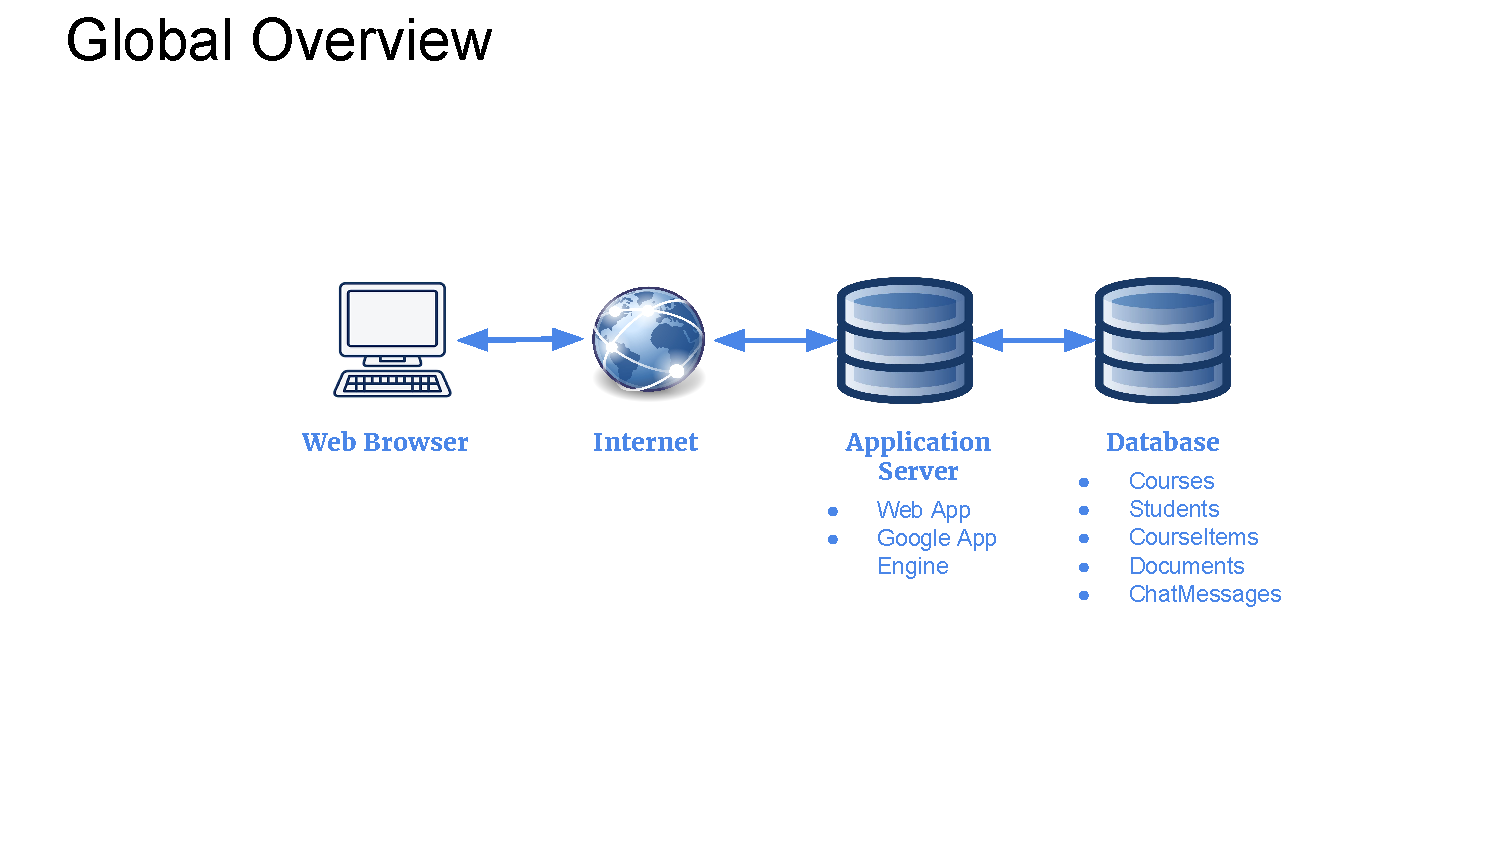
\includegraphics[page=1,width=0.9\textwidth]{diagrams/SDD_Diagrams.pdf}
  \label{fig:SDD_1}
\end{figure}

\begin{figure}[ht]
  \centering
  \includegraphics[page=2,width=0.9\textwidth]{diagrams/SDD_Diagrams.pdf}
  \label{fig:SDD_1}
\end{figure}

\begin{figure}[ht]
  \centering
  \includegraphics[page=3,width=0.9\textwidth]{diagrams/SDD_Diagrams.pdf}
  \label{fig:SDD_1}
\end{figure}

\section{Description of Achitecture Goals}
The Class Collaboration Application will be hosted by the Google App Engine and users will access the app via a web browser. The app will have access to a database containing lists of all the Courses created for the app, corresponding CourseItems, Documents, and Chatmessages, as well as the Students who have created accounts. The database will save the information for an indefinite amount of time. Our class structures and main use cases by users are shown below. 

\section{Design Rationale}
\hspace{10mm}We have decided to use Google App Engine because it is a reliable platform to scale and build web applications. Many web applications are maintained either through IaaS or PaaS. We decided not to use Iaas because, although we can have root access to a VM, we would have to be responsible for managing the resources on the machine including, memory and CPU usage. Since Google App Engine is a PaaS, it manages all of our computational resources for us, so our only responsibility is maintaining the application while Google App Engine would take care of the infrastructure, security and scalability of the Class Collaboration Application. 

\hspace{10mm}For each user, we decided to integrate SSO into our application. Using SSO as a way for users to sign into the application through their Case credentials boosts our security capabilities as well as mitigates the risk of 3rd party applications accessing sensitive information about the user. This also improves user experience since the user does not have to create and keep track of another username and password. 


%%%%%%%%%%%%%%%%%%%%%
% PRINCIPAL Components %
%%%%%%%%%%%%%%%%%%%%%

\chapter{Principal Components}
	
\section{Component:User Info Management}
\subsection{Component Description}
Users who use the platform for the first time need to register first. After successful registration, the system will jump to the login page. Users log in to the system through a valid user name and password, and then jump to the home page.\\

\noindent When users view their personal information on the personal page, they need to obtain the information saved in the database. Modifying personal information also needs to submit the modified information to the database of iSport.\\

\noindent All the above behaviors must interact with the database and blockchain to obtain and change the corresponding user personal information. The call relationship between classes is shown in the figure below:
\begin{figure}[H]
	\centering
	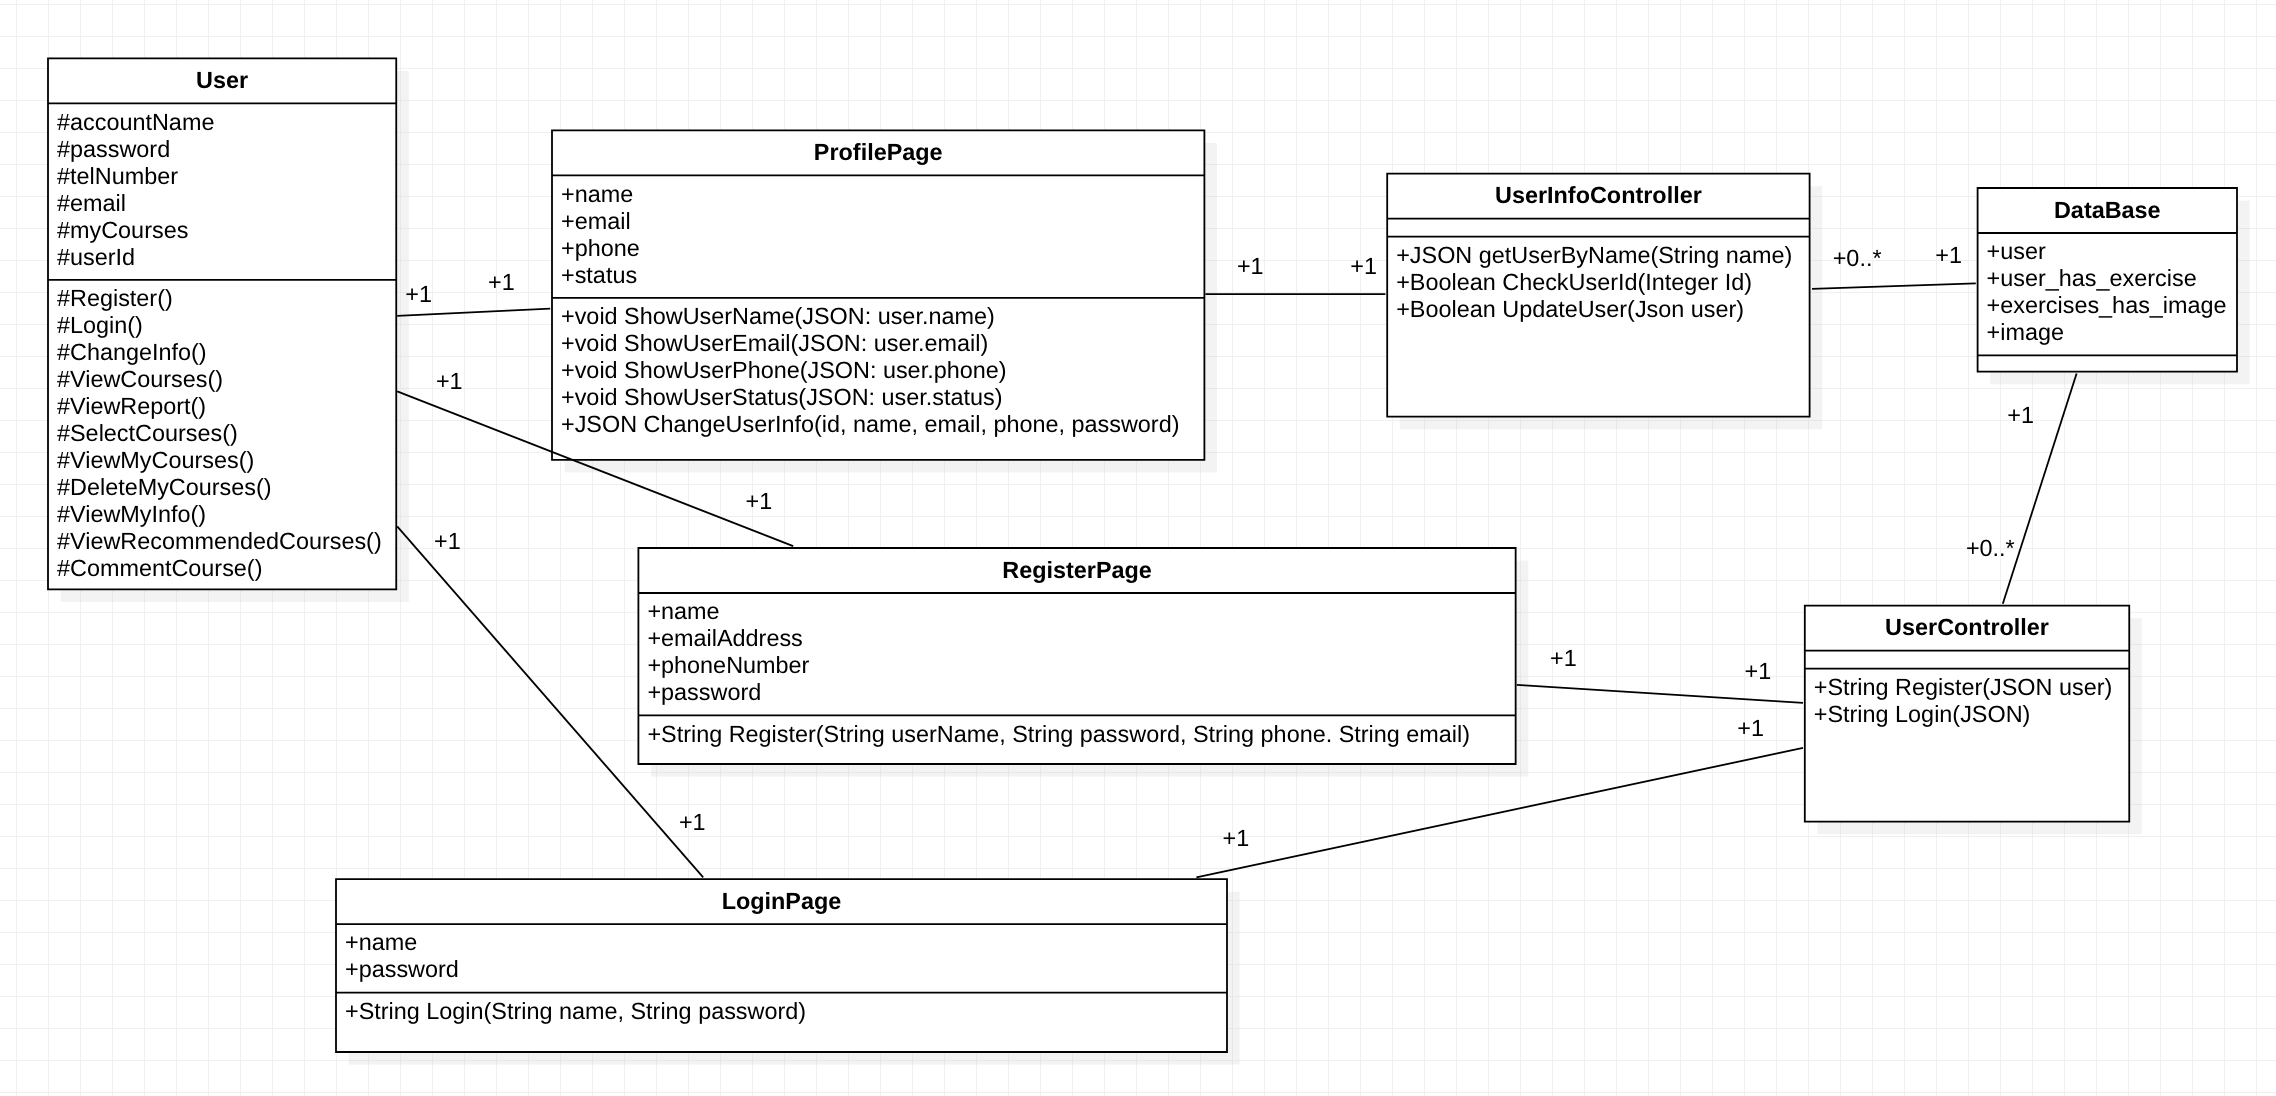
\includegraphics[width=1.0\textwidth]{diagrams/userinfo.png}
	\caption{Class Diagram of UserInfo Component}
\end{figure}
\subsection{Responsibilities}
\begin{itemize}
	\item User can register through UserInfo Component.
	\item User can login iSport by UserInfo Component. 
	\item User can check his/her information through UserInfo Component on Profile Page. 
	\item User can update his/her information through UserInfo Component on Profile Page. 
\end{itemize}

\subsection{Component Design Detail Description}
\subsubsection{Design for User Login in}
\begin{itemize}
	\item Input: User Name; User Password
	\item Output: Whether the user log in successfully
	\item Logical Flow:
	 \begin{figure}[H]
	\centering
	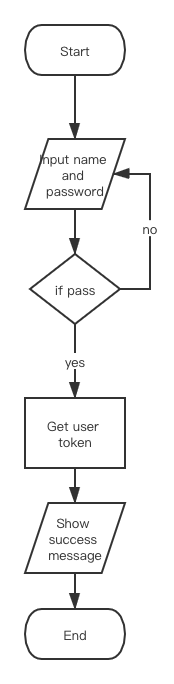
\includegraphics[width=0.2\textwidth]{diagrams/login.png}
	\caption{Logical Flow for User Log in}
\end{figure}
	\item Interface Design
	\begin{center}
    \begin{tabular}{p{5cm}p{10cm}}
        \hline
	    Request Method & Post\\
        \hline
	    Service Routing &  http://[host]:6060/user/login\\
        \hline
	    Params & \makecell[l]{Params1: user name;\\ Params2: user password;\\ Params3: request}\\ 
        \hline
        Params Type & \makecell[l]{user name: String;\\user password:String;\\ request: HttpServletRequest}\\
        \hline
        Description & Check if the user's password is right according to the input user name and password.\\
        \hline
        Return Type & Json.\\
        \hline
    \end{tabular}
\end{center}
\item Restriction and Error Handling\\
\begin{enumerate}
	\item User has registered before.
\end{enumerate} 
\end{itemize}

\subsubsection{Design for User Register}
\begin{itemize}
	\item Input: \\
	\begin{enumerate}
		\item User Name : Got by HttpRequest (compulsory)
		\item User Password: Got by HttpRequest (compulsory)
		\item Email Address: Got by HttpRequest (compulsory)
		\item Phone Number: Got by HttpRequest (compulsory)
	\end{enumerate}
	\item Output: Whether the user register successfully
	\item Logical Flow:
	 \begin{figure}[H]
	\centering
	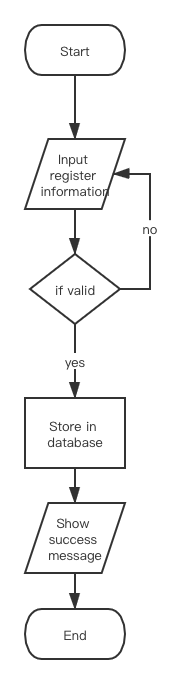
\includegraphics[width=0.2\textwidth]{diagrams/register.png}
	\caption{Logical Flow for User Register}
\end{figure}
	\item Interface Design
	\begin{center}
    \begin{tabular}{p{5cm}p{10cm}}
        \hline
	    Request Method & Post\\
        \hline
	    Service Routing &  http://[host]:6060/user/register\\
        \hline
	    Params & \makecell[l]{Params1: user name;\\ Params2: user password;\\ Params3: phone;\\Params4: email}\\ 
        \hline
        Params Type & \makecell[l]{user name: String;\\user password:String;\\ phone: String;\\email: String}\\
        \hline
        Description & Help the user register iSport.\\
        \hline
        Return Type & Json.\\
        \hline
    \end{tabular}
\end{center}
\item Restriction and Error Handling\\
\begin{enumerate}
	\item User has related information to register iSport.
\end{enumerate} 
\end{itemize}

\subsubsection{Design for User Check Personal Information}
\begin{itemize}
	\item Input: null
	\item Output: User's profile page
	\item Logical Flow:
	 \begin{figure}[H]
	\centering
	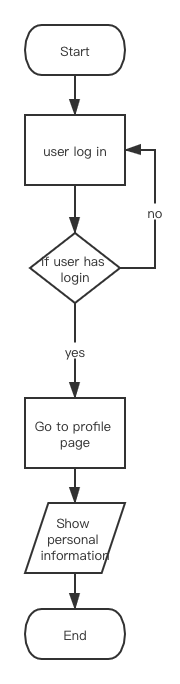
\includegraphics[width=0.2\textwidth]{diagrams/checkuserinfo.png}
	\caption{Logical Flow for User Checking Info}
\end{figure}
	\item Interface Design
	\begin{center}
    \begin{tabular}{p{5cm}p{10cm}}
        \hline
	    Request Method & GET\\
        \hline
	    Service Routing &  http://[host]:6060/{userName}/info\\
        \hline
	    Params & \makecell[l]{Params1: user name}\\ 
        \hline
        Params Type & \makecell[l]{user name: String}\\
        \hline
        Description & Get user's information and show on the profile page.\\
        \hline
        Return Type & Json.\\
        \hline
    \end{tabular}
\end{center}
\item Restriction and Error Handling\\
\begin{enumerate}
	\item User has personal information stored in database.
\end{enumerate} 
\end{itemize}

\subsubsection{Design for User Update Personal Information}
\begin{itemize}
	\item Input: 
	\begin{enumerate}
		\item user name
		\item user password
		\item email
		\item phone
	\end{enumerate}
	\item Output: User's profile page
	\item Logical Flow:
	 \begin{figure}[H]
	\centering
	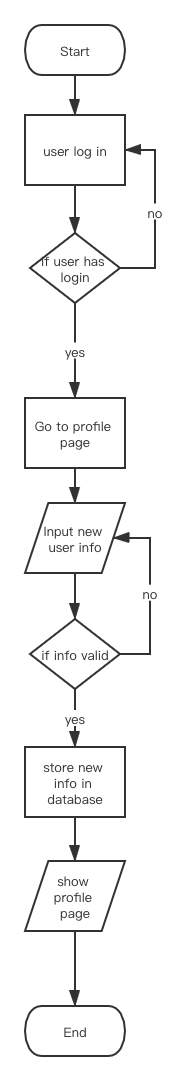
\includegraphics[width=0.2\textwidth]{diagrams/updateinfo.png}
	\caption{Logical Flow for User Updating Info}
\end{figure}
	\item Interface Design
	\begin{center}
    \begin{tabular}{p{5cm}p{10cm}}
        \hline
	    Request Method & GET\\
        \hline
	    Service Routing &  http://[host]:6060/{userId}/updateInfo\\
        \hline
	    Params & \makecell[l]{Params1: user id;\\Params2: user name;\\Params3: email;\\Params4: tel;\\Params5: password}\\ 
        \hline
        Params Type & \makecell[l]{user id: Integer;\\user name: String;\\email: String;\\tel: String\\password: String}\\
        \hline
        Description & Update user's information and refresh the profile page.\\
        \hline
        Return Type & Json.\\
        \hline
    \end{tabular}
\end{center}
\item Restriction and Error Handling\\
\begin{enumerate}
	\item User has personal information stored in database.
	\item User provide valid new personal information.
\end{enumerate} 
\end{itemize}

\section{Component:User Postures Detection}
\subsection{Component Description}
When the user start to exercise, he/she have to stand before the camera and Detection component will open the camera and show the user's posture video in real time. \\

\noindent And then this component will get the user's key points positions by using PoseNet, and draw the user's skeleton according to theses key points.\\

\noindent The call relationship between classes is shown in the figure below:
\begin{figure}[H]
	\centering
	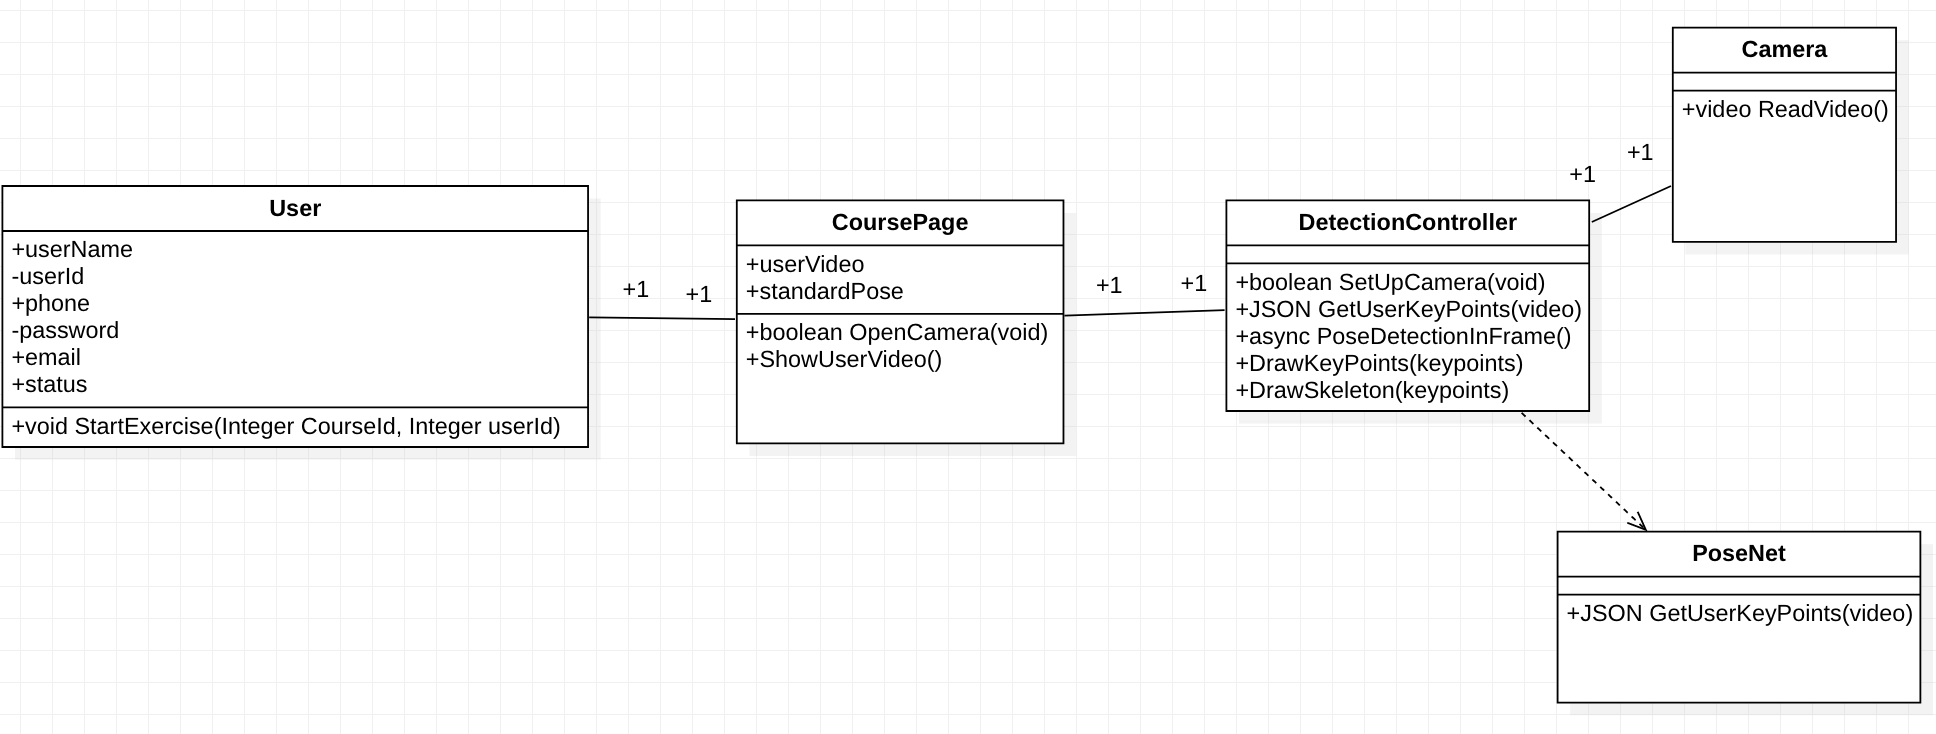
\includegraphics[width=1.0\textwidth]{diagrams/detection.png}
	\caption{Class Diagram of Detection Component}
\end{figure}
\subsection{Responsibilities}
\begin{itemize}
	\item Set up the camera, record and show user's video.
	\item Get user posture key points and draw the skeleton. 
\end{itemize}

\subsection{Component Design Detail Description}
\subsubsection{Design for Video, KeyPoints Reading and Playing}
\begin{itemize}
	\item Input: null
	\item Output: User's video
	\item Logical Flow:
	 \begin{figure}[H]
	\centering
	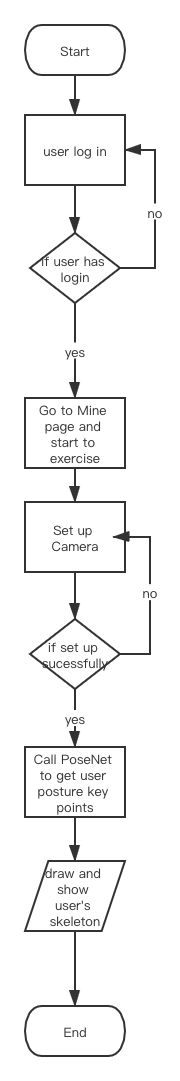
\includegraphics[width=0.2\textwidth]{diagrams/video.png}
	\caption{Logical Flow for Video Setup and KeyPoints Reading}
\end{figure}
	\item Function Design
	\begin{center}
    \begin{tabular}{p{6cm}p{10cm}}
        
        \hline
	    setupCamera & \makecell[l]{Params: null;\\Return Type:async function;\\Function: Apply authority to user camera.}\\ 
        \hline
        loadVideo & \makecell[l]{Params: null;\\Return Type:async function;\\Function: Apply authority to user camera.}\\ 
        \hline
        detectionPoseInRealTime & \makecell[l]{Params: video;\\Return Type: async function;\\Function:play the user video}\\
        \hline
        bindPage &  \makecell[l]{Params: null\\Return Type: async function;\\Function:load the poseNet model}\\
        \hline
        PoseDetectionFrame & \makecell[l]{Params: null\\Return Type: async function;\\Function:use the poseNet model to detect \\every frame's keypoints}\\
        \hline
        drawKeyPoints & \makecell[l]{Params: keypoints\\Return Type: void;\\Function:to draw the keypoints which \\PosetNet read}\\
        \hline
        drawSkeleton & \makecell[l]{Params: keypoints\\Return Type: void;\\Function:to draw the skeleton according to \\the keypoints}\\
        \hline
    \end{tabular}
\end{center}
\item Restriction and Error Handling\\
\begin{enumerate}
	\item User has logged in.
	\item The camera works well.
\end{enumerate} 
\end{itemize}


%\section{Course}
%A Course class is able to aggregate all of the information and student created objects that are associated with a particular course. Created objects include all of the CourseItem objects associated with the Course and a single Chat object to be used as the general chat for the Course.
%\subsection{Responsibilities}
%\begin{itemize}
%	\item Presenting to the user all CourseItem objects that have been added to the course from all Students 
%	\item Presenting the Chat object for the course to allow communication between the Student and all other Students with the chat object
%	\item Querying any updates to the Course objects and updating the CourseItem and Chat objects
%\end{itemize}
%
%
%
%\section{CourseItem}
%A Course Item class is a reference to an assignment, exam, URL, or other document relevant to the course. The object in code will serve as a container and mainly server metadata information, while the document itself will be stored in the database. The CourseItem is a created object that is created by a user in the Student class and will be shared through a Course’s chat object and always accessible on the sidebar. The user who created the CourseItem object will be able to later modify or delete the object.
%\subsection{Responsibilities}
%\begin{itemize}
%	\item Display to the user the name and description of the courseItem
%	\item Allow the creator of the courseItem to modify or delete the courseItem
%	\item Query any updates to the courseItem and update the courseItem accordingly
%	\item Provide a download option so that a Student can download the contents of a course item
%\end{itemize}
%
%\section{Chat}
%A chat is created for each Course and for each CourseItem. Chats are not created by or associated with users in any way, they are only automatically created/exist alongside existing Courses and CourseItems.
%\subsection{Responsibilities}
%\begin{itemize}
%	\item Tracking and recording to the database new messages in the chat. Messages are written to the database immediately (are not written to a buffer/flushed).
%	\item Notifying the client of changes when the client checks (asks) whether any changes (new messages) have occurred.
%	\item Providing specific messages upon request.
%	\item Caching messages as they are accessed to reduce read operations on the database.
%	\item Displaying active and offline users of chat channel
%\end{itemize}
%%%%%%%%%%%%%%%%%%%%
% CLASS INTERFACES %
%%%%%%%%%%%%%%%%%%%%

\chapter{Class Interfaces}

\section{Classes of User Info Management Component}

\subsection{Class UserController}
\subsubsection{Attribute Description}
null
\subsubsection{Methods Description}
\begin{enumerate}
	\item getUserName(userId): String
	\begin{enumerate}
		\item Parameters: Integer userId
		\item Return Type: String
		\item Function: According to the input userId, check if the userId exists, if userId doesn't exist output "Id don't exist", otherwise,return the name of the user with the corresponding id.
		\item Detail Description: To find the user name with corresponding userId in table user of the database.
		\item Implement:
		\begin{figure}[H]
	\centering
	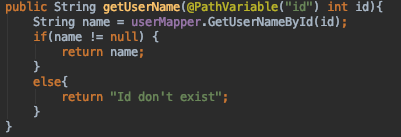
\includegraphics[width=0.7\textwidth]{diagrams/getusername1.png}\\
\end{figure}
	\end{enumerate}
	\item getUserInfo(userName): User
	\begin{enumerate}
		\item Parameters: String userName
		\item Return Type: User
		\item Function: According to the input userName, check if the userName exists and return the corresponding user info.
		\item Detail Description: To find the user info(name, phone, email, status) with corresponding userName in table user of the database.
		\item Implement:
		\begin{figure}[H]
	\centering
	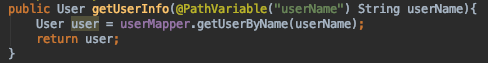
\includegraphics[width=0.8\textwidth]{diagrams/getuserinfo.png}\\
\end{figure}
	\end{enumerate}
	\item register
	\begin{enumerate}
		\item Parameters: userName, password, phone, email
		\item Return Type: String
		\item Function: Register an account for user, and store the user info in database. But check if there is already a same user name first.
		\item Detail Description: To store the user info(name, phone, email, status) in database.
		\item Implement:
		\begin{figure}[H]
	\centering
	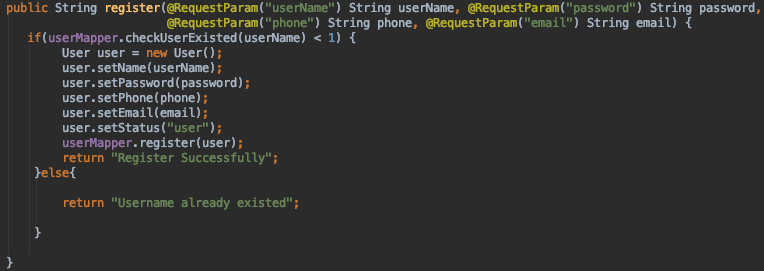
\includegraphics[width=0.9\textwidth]{diagrams/registerfunc.png}\\
\end{figure}
\end{enumerate}
	\item login
	\begin{enumerate}
		\item Parameters: userName, password
		\item Return Type: String
		\item Function: According to the input userName and password check if the user can login iSport successfully.
		\item Detail Description: Find the record in table user with corresponding userName and password.
		\item Implement:
		\begin{figure}[H]
	\centering
	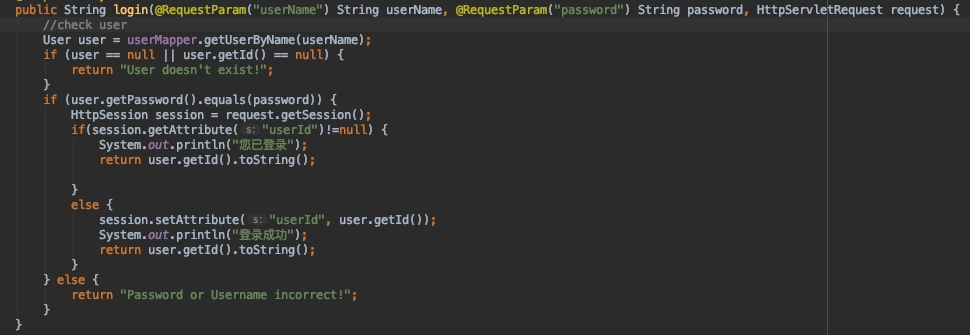
\includegraphics[width=0.9\textwidth]{diagrams/loginfunc.png}\\
\end{figure}
\end{enumerate}
	\item updateUserInfo
	\begin{enumerate}
		\item Parameters: userId, userName, email, tel, password
		\item Return Type: String
		\item Function: According to the input user info to update the user's information.
		\item Detail Description: Find the record in table user with corresponding userId and update the related info.
		\item Implement:
		\begin{figure}[H]
	\centering
	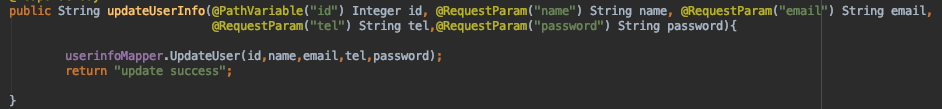
\includegraphics[width=1.\textwidth]{diagrams/updateinfofunc.png}\\
\end{figure}
	\end{enumerate}
\end{enumerate}



 

%%%%%%%%%%%%%%%%%%%%%%%%%%
% HUMAN INTERFACE DESIGN %
%%%%%%%%%%%%%%%%%%%%%%%%%%

\chapter{Human Interface Design}

\section{Mockup of User Interface}

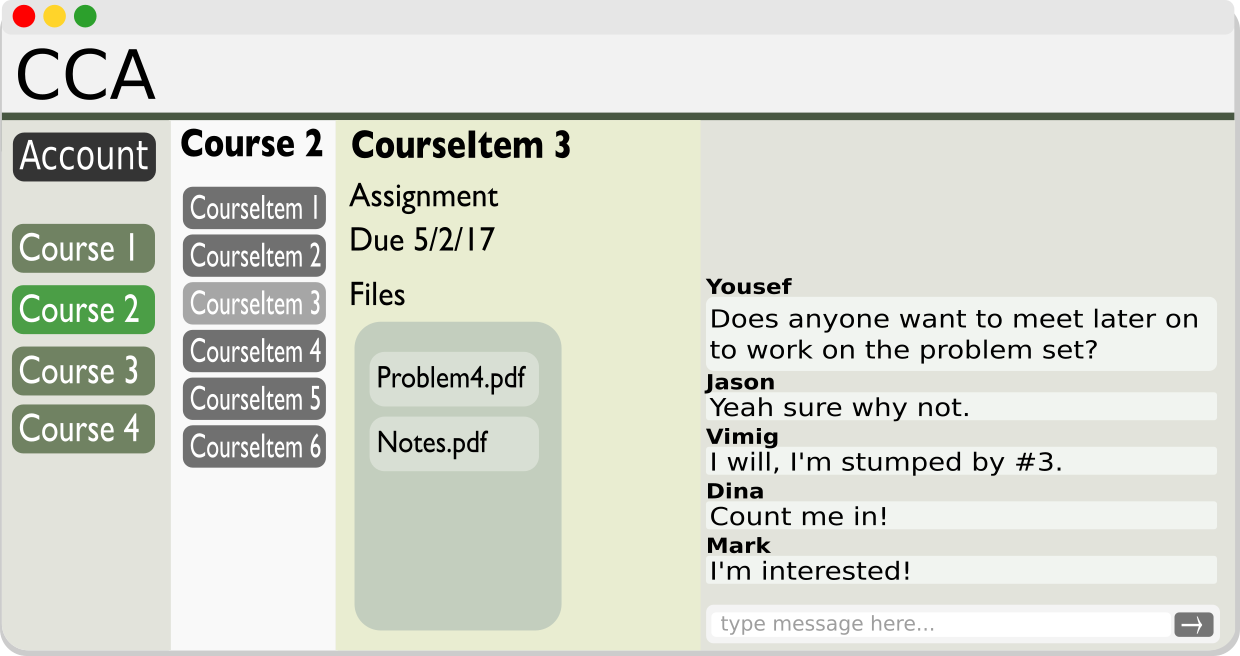
\includegraphics[width=1.0\textwidth]{diagrams/UI_Mockup.png}


\end{document}
